% \input{"//iab.baintern.de/Dfs/017/Ablagen/D01700-Info-Board/06_WMK/Corporate Design/Folienvorlagen/TeX-Folienformat.tex"}
\input{"/Users/jonathanlatner/Google Drive/My Drive/IAB/latex/TeX-Folienformat.tex"}


\documentclass[t,8pt,utfx8]{beamer}
\usepackage{booktabs}
\usepackage{setspace}
\usepackage{parskip}
\setbeamertemplate{caption}[numbered]
\newcommand{\sprache}{\englisch}
\renewcommand{\thesubsection}{\alph{subsection})}

\newcommand{\btVFill}{\vskip0pt plus 1filll}

\title[Balancing Data Utility and Privacy: Evaluating Computer Science and Statistical approaches to Synthetic Data]{Balancing Data Utility and Privacy: Evaluating Computer Science and Statistical approaches to Synthetic Data}
\subtitle{DiskAB, 19. Juni, 2023}

\author{Jonathan Latner, PhD \newline Prof. Dr. Jörg Drechsler}

\newcounter{noauthorlines}
\setcounter{noauthorlines}{2} % Wert für 2 Autoren über 2 Zeilen. Ggf. anpassen

% %%%%%%%%%%%%%%
% Ende Anpassung
% %%%%%%%%%%%%%%

% \input{"//iab.baintern.de/Dfs/017/Ablagen/D01700-Info-Board/06_WMK/Corporate Design/Folienvorlagen/TeX-Folienformatierung_CD_2019"}
\input{"/Users/jonathanlatner/Google Drive/My Drive/IAB/latex/TeX-Folienformatierung_CD_2019"}

% Modify the section in toc template to enumerate
\setbeamertemplate{section in toc}{%
    \inserttocsectionnumber.~\inserttocsection\par
}

% use for subsections
\setbeamertemplate{subsection in toc}{}
% \setbeamertemplate{subsection in toc}{%
%     \setlength{\parskip}{1mm}
%     %     \hskip2mm -- \hskip1mm\inserttocsubsection\par
% }

\titlegraphic{\includegraphics[width=2cm]{/Users/jonathanlatner/Google Drive/My Drive/IAB/latex/CD 2019/aniged.png}}

\begin{document}


\section{Background}\label{sec_intro}
\frame[plain]{\titlepage}

\begin{spacing}{1.25}

%Table of contents
\begin{frame}
\frametitle{Sections}
\vskip6mm
\setlength{\leftskip}{0.5mm}
\setlength{\parskip}{5mm}
\begin{NoHyper}
        \tableofcontents
\end{NoHyper}
\end{frame}

\frame[c]{\frametitle{}
\centering
Section \ref{sec_intro}: Introduction
}



\frame{\frametitle{What is the background?}
\begin{itemize}
    \item Synthetic data are data that mimic the characteristics of original or `real' data, but are not derived from actual observations or measurements.
    \item Synthetic data is appealing because it looks like real data, but without any of the threats to privacy contained in real data.
    \item With no risk to privacy, more data could be released, accessed more easily, and more knowledge could be created (i.e. firm-level, administrative, tax data, health records, etc.).
    \item In 1993, Rubin proposed the idea of releasing synthetic data instead of the real data.
    \item Since then, different approaches for the generation of synthetic data have been developed.
    \item The goal: any analysis run on the synthetic data should provide approximately the same answers that would have been obtained if the analysis were run on the original data.
    \begin{itemize}
                \item In statistics, emphasis is on reducing privacy risk while maintaining (or increasing!) utility (i.e. Parametric/CART)
        \item In computer science, emphasis is a general approach to many different types of data (i.e. images) - (Bayes/GANs)
    \end{itemize}

\end{itemize}
}

\frame{\frametitle{What is the goal?}
\begin{itemize}
    \item Evaluate how suitable the computer science approaches to synthetic data are from a statistical perspective. 
    \item Compare and contrast the how different approaches balance the twin goals of data utility and data privacy.
    \item In this talk, we will present some first results from this project.
    \item For now, we focus on utility (next steps: privacy)  
\end{itemize}
}

\frame{\frametitle{Comparing different packages for creating synthetic data}
\begin{itemize}
        \item Most papers are often written by the package authors
    \begin{itemize}
                \item In these papers, their package is often the `winner'
        \item This is not necessarily wrong
        \item This is a reflection of different strengths and weaknesses
    \end{itemize}
    \item Few `independent' papers compare and contrast
    \begin{itemize}
                \item Little et al., 2021/2023 ({\emph Working paper})
        \begin{itemize}
                        \item They don't tune the packages
            \item They primarily rely on data sets with mostly categorical data and incorrectly claim that (2023), `Census microdata is predominantly categorical...' 
        \end{itemize}
        \item Dankar and Ibrahim (2021)
        \begin{itemize}
                        \item They do tune, but not clear how.
        \end{itemize}
    \end{itemize}
\end{itemize}
}

\frame{\frametitle{Preview results}
\begin{itemize}
        \item Main message: Synthpop is the `winner'
    \begin{itemize}
                \item However, it is not always the `best'
        \item Easy - little tuning required 
        \item Fastest
    \end{itemize}
    \item Datasynthesizer
    \begin{itemize}
                \item Requires tuning
        \item Struggles with continuous variables
    \end{itemize}
    \item CTGAN
    \begin{itemize}
                \item Requires tuning
        \item Struggles with categorical variables
        \item Slowest
    \end{itemize}
\end{itemize}
}

\section{Data}\label{sec_data}
\frame[c]{\frametitle{}
\centering
Section \ref{sec_data}: Data
}

\frame{\frametitle{Data}
\begin{itemize}
    \item 2 simulated data sets
    \begin{itemize}
        \item Isolate differences between synthetic data packages and the effect of tuning hyperparameters in a `controlled' environment 
    \end{itemize}
    \item 2 real data sets
    \begin{itemize}
        \item Benchmark our results to published papers using these data
    \end{itemize}
    \item Others (next steps)
\end{itemize}
}

\frame{\frametitle{Simulated data}
\begin{itemize}
    \item Categorical data
    \begin{itemize}
        \item 4 bivariate categorical variables (`Y', `N')
        \item 1.000 observations
    \end{itemize}
    \item Simulated continuous data
    \begin{itemize}
        \item 3 continuous variables (`income', `wealth', `age')
        \item 1.000 observations
    \end{itemize}
\end{itemize}
}

\frame{\frametitle{Real data}
\begin{itemize}
    \item UK 1991: Individual Sample of Anonymised Records (SAR) for the British Census, subsetted on the region of West Midlands
    \begin{itemize}
        \item 20\% sample ($\approx 20.000$)
        \item 12 variables: 1 numerical and 11 categorical, includes missing values
        \item Used by Little et al., 2021/2023
    \end{itemize}
    \item SD 2011: Social Diagnosis 2011 - Objective and Subjective Quality of Life in Poland
    \begin{itemize}
        \item 5.000 observations
        \item 4 variables: 2 numerical (`age', `income') and 2 categorical (`edu', `sex'), includes missing values
        \item Used by Synthpop package
    \end{itemize}
\end{itemize}
}


\section{Methods}\label{sec_methods}
\frame[c]{\frametitle{}
\centering
Section \ref{sec_methods}: Methods
}

\frame{\frametitle{Methods}
\begin{itemize}
        \item Compare 3 packages for creating synthetic data sets
    \begin{itemize}
            \item CTGAN (Conditional Tabular Generative Adversarial Network) in Synthetic Data Vault (SDV) package  (Patki et al., 2016)
        \item Datasynthesizer (Ping et al., 2017)
        \item Synthpop (Nowak et al., 2016)
    \end{itemize}
    \item We choose these three because they are commonly compared (Little et al., 2021/2023; Dankar and Ibrahim, 2021)
    \item Other packages (next steps)
\end{itemize}
}


\frame{\frametitle{Comparison}
Different strengths and weaknesses
\begin{table}[h]
\caption{Comparison of data synthesis packages}
\label{table_comparison}
\centering
\vskip -5mm
\begin{tabular}{lccc}
\toprule
Variable/data & CTGAN (GANs) & Datasynthesizer (PrivBayes) & Synthpop (CART) \\
\midrule
Continuous variables & \checkmark & & \checkmark\\
Categorical variables & & & \checkmark \\
Mixed data & & \checkmark & \checkmark \\
Privacy protection & \checkmark$^*$ & \checkmark & \\
Relational datasets & \checkmark & & \\
High dimensional datasets & & \checkmark & \\
\bottomrule
\multicolumn{4}{p{14cm}} {\footnotesize $^*$ In theory, GANs reduce disclosure risk because they do not access the original (or training) data at all, and starts off with only noise as input.  This is also why they should be superior for continuous variables.}
\end{tabular}
\end{table}

}


\section{Tuning}\label{sec_tuning}
\frame[c]{\frametitle{}
\centering
Section \ref{sec_tuning}: Tuning
}

\frame{\frametitle{CTGAN}
\begin{itemize}
    \item A total of 11 hyperparameters can be tuned, we focus on 4$^*$
    \begin{itemize}
        \item {\bf epochs} (3: 300, 600, 900): the number of iterations that the model will perform to optimize its parameters. Default is 300.  
        \item {\bf discriminator\_steps} (3: 1, 5, 10): Number of discriminator updates to do for each generator update. Default is 1.
        \item {\bf batch\_size} (2: 500, 1000): as well as the number of samples used in each step. Default is 500.  
        \item {\bf log\_frequency} (2: True, False): Whether to use log frequency of categorical levels in conditional sampling. It defaults to True. This argument affects how the model processes the frequencies of the categorical values that are used to condition the rest of the values. In some cases, changing it to False could lead to better performance.
    \end{itemize}
    \item copies (3: 1, 5, 10): Number of synthetic data sets
    \item Total: 108 combinations of tuning parameters (576 synthetic data sets)
\end{itemize}

\btVFill
\tiny

Source: \url{https://sdv.dev/SDV/user_guides/single_table/ctgan.html\#advanced-usage} \\
\url{https://docs.sdv.dev/sdv/single-table-data/modeling/synthesizers/ctgansynthesizer} \\
$^*$We don't use `discriminator\_dim', `discriminator\_decay', `discriminator\_lr', `embedding\_dim', `generator\_decay', `generator\_dim', `generator\_lr', `pac'


}

\frame{\frametitle{Datasynthesizer}
\begin{itemize}
    \item A total of 11 hyperparameters can be tuned, but we focus on 2$^*$
    \begin{enumerate}
        \item {\bf k} (3: 0, 1, 2).  The maximum number of parents in Bayesian network, i.e., the maximum number of incoming edges.  Default is 0.
        \item {\bf $\epsilon$} (7: 0, 0.1, 1, 5, 10, 20, 30).  It roughly means that removing a row in the input dataset will not change the probability of getting the same output more than a multiplicative difference of exp($\epsilon$).  Set $\epsilon$=0 to turn off differential privacy.  Default is 0.1.  Epsilon value usually are less than one, but it’s not uncommon to see larger $\epsilon$ being used (i.e. U.S. Census is 19.61).$^\dagger$
    \end{enumerate}
    \item copies (3: 1, 5, 10): Number of synthetic data sets
    \item Total: 63 combinations of tuning parameters (336 synthetic data sets)
\end{itemize}

\btVFill
\tiny

Source: \url{https://github.com/DataResponsibly/DataSynthesizer/blob/master/DataSynthesizer/DataDescriber.py} \\
$^*$ Others available, but relate to dictionaries (`category\_threshold', `null\_values', `attr\_to\_datatype', `attr\_to\_is\_categorical', `attr\_to\_is\_candidate\_key', etc.) \\
$^\dagger$ \url{https://www.ncsl.org/health/differential-privacy-for-census-data-explained} 

}

\frame{\frametitle{Synthpop}
\begin{itemize}
    \item Many hyperparameters can be tuned, but we focus on 2$^*$
    \begin{enumerate}
        \item  {\bf complexity parameter} (5: 1e-8, 1e-6, 1e-4, 0.01).  Any split that does not decrease the overall lack of fit by a factor of cp is not attempted. Small values of cp will grow large trees.  Default is 0.00000001 (1e-8).
        \item {\bf minbucket} (4: 5, 10, 25, 50). the minimum number of observations in any terminal $<leaf>$ node. Default is 5.  
    \end{enumerate}
    \item copies (3: 1, 5, 10): Number of synthetic data sets
    \item Total: 48 combinations of tuning parameters (256 synthetic data sets)
\end{itemize}

\btVFill
\tiny

Source: \url[pg. 10-11]{https://cran.r-project.org/web/packages/synthpop/vignettes/utility.pdf} \\
\url{https://alfurka.github.io/2023-01-30-creating-synthetic-values-with-synthepop-cart/} \\
$^*$ Others available, but relate to dictionaries (minnumlevels, cont.na, etc.).  We don't use `proper' or `smoothing', at least not yet.


}

\section{Measuring utility}\label{sec_utility}
\frame[c]{\frametitle{}
\centering
Section \ref{sec_utility}: Measuring utility \\
}

\frame{\frametitle{Measuring utility}

\begin{itemize}
    \item Ratio of estimates (ROE)$^*$ 
    \begin{itemize}
        \item The ratio of the synthetic and original data estimates (e.g. totals, proportions), where the smaller of these two estimates is divided by the larger one. Max = 1, min = 0, higher is better.  If $y^1_{orig}$ = $y^1_{synth}$, then ROE = 1.  Continuous variables are binned (20).  
        \item The ROE is calculated over univariate and  bivariate values of a given variable(s).  
    \end{itemize}
    \item Difference/overlap in the estimate/confidence interval$^\dagger$
    \begin{itemize}
        \item Standardized difference (Std. Diff) - the absolute value of the difference between the coefficients from the same regression model applied to original and synthetic data, divided by the standard error of the estimate from the model applied to original data.  Lower is better (closer to 0).
        \item Confidence interval overlap (CIO) - the \% overlap between the confidence interval of a given point estimate from the same regression model applied to original and synthetic data.  Higher CIO indicates greater utility.  Maximum value is 1, negative value indicating no overlap (here, negative = 0).
    \end{itemize}
    \item Others (next steps)
\end{itemize}
\btVFill
\tiny

$^*$ \url{https://github.com/clairelittle/psd2022-comparing-utility-risk/blob/main/code/ROC_Ratio_of_Counts_Estimates.R} \\
$^\dagger$ \url{https://github.com/clairelittle/psd2022-comparing-utility-risk/blob/main/code/CIO_Confidence_Interval_Overlap.R}

}


% To calculate the Confidence interval overlap (CIO), using 95\% confidence intervals, the coefficients from regression models built on the original and synthetic datasets are used. The CIO, proposed by Karr et al., 2006, is defined as:


% \frame{\frametitle{Ratio of estimates (ROE)}

% The ratio of estimates (ROE) is the ratio of the synthetic and original data estimates (e.g. totals, proportions), where the smaller of these two estimates is divided by the larger one. Thus, given two corresponding estimates, where $y^1_{orig}$ is the estimate from the original data and $y^1_{synth}$ is the corresponding estimate from the synthetic data, and is calculated as:

% \begin{equation}
%     ROE = \frac{min(y^1_{orig},y^1_{synth})}{max(y^1_{orig},y^1_{synth})}
% \end{equation}

% Max = 1, min = 0, higher is better.  If $y^1_{orig}$ = $y^1_{synth}$, then ROE = 1.  Continuous variables are cut into bins of 20.  The ROE is calculated over bivariate and univariate data.  

% \begin{table}[!h]
%     \input{../../support_files/tables/table_roe_example.tex}
%     \label{table_roe_example}
% \end{table}

% \btVFill
% \tiny

% Source: \url{https://github.com/clairelittle/psd2022-comparing-utility-risk/blob/main/code/ROC_Ratio_of_Counts_Estimates.R}

% }

% \frame{\frametitle{Standardized difference}

% Standardized difference (Std. Diff) is the absolute value of the difference between the coefficients from the same regression model applied to original and synthetic data, divided by the standard error of the estimate from the model applied to original data: 

% \vskip -5mm
% \begin{equation}
%     \text{Std. Diff.} = \frac{\left|\beta_o - \beta_s\right|}{\sigma_o}
% \end{equation}

% \begin{figure}
%     \resizebox{\textwidth}{!}{\includegraphics{../../support_files/graphs/graph_cio_example.pdf}}
%     \label{graph_cio_example}
% \end{figure}

% \vskip -5mm
% \begin{table}[!h]
%     \input{../../support_files/tables/table_cio_example_std.tex}
%     \label{table_cio_example_std}
% \end{table}

% \btVFill
% \tiny

% Source: \url{https://github.com/clairelittle/psd2022-comparing-utility-risk/blob/main/code/CIO_Confidence_Interval_Overlap.R}

% }

% \frame{\frametitle{Confidence interval overlap (CIO)}

% To calculate the Confidence interval overlap (CIO), using 95\% confidence intervals, the coefficients from regression models built on the original and synthetic datasets are used. The CIO, proposed by Karr et al., 2006, is defined as:

% \vskip -3mm
% \begin{equation}
%     CIO = \frac{1}{2}\left\{\frac{min(\mu_o,\mu_s)-max(l_o,l_s)}{\mu_o - l_o} + \frac{min(\mu_o,\mu_s)-max(l_o,l_s)}{\mu_s - l_s}\right\}
% \end{equation}

% where $\mu_o, l_o, l_s$ denote the respective upper and lower bounds of the confidence intervals for the original and synthetic data.  Higher CIO indicates greater utility.  Maximum value is 1, negative value indicating no overlap (here, negative = 0).

% \begin{figure}
%     \resizebox{\textwidth}{!}{\includegraphics{../../support_files/graphs/graph_cio_example.pdf}}
%     \label{graph_cio_example}
% \end{figure}

% \vskip -6mm
% \begin{table}[!h]
%     \input{../../support_files/tables/table_cio_example_cio.tex}
%     \label{table_cio_example_cio}
% \end{table}


% \btVFill
% \tiny

% Source: \url{https://github.com/clairelittle/psd2022-comparing-utility-risk/blob/main/code/CIO_Confidence_Interval_Overlap.R}

% }

% \frame{\frametitle{CIO - How do we decide the right parametric model to use?}

% Research choice - there is no one, right way
% \begin{itemize}
%     \item GLM/LPM
%     \item In categorical variables, what is dependent value?
%     \item Theoretical/atheoretical models
%     \begin{itemize}
%         \item `Atheoretical' models are where each variables is DV and all other variables are IV
%         \item `Theoretical' models make informed choices about DV/IVs 
%     \end{itemize}
% \end{itemize}

% Here, it depends on the data source:
% \begin{itemize}
%     \item Simulated categorical - atheoretical
%     \item Simulated continuous - atheoretical
% \end{itemize}

% }

\frame{\frametitle{Methods}

For each package (Datasynthesizer, CTGAN, Synthpop), estimate the effect of each categorical hyperparameters ($h$) on each utility measure ($y_i$) (ROE\_u, ROE\_b, Std. Diff, and CIO) in model \ref{model_1} and for each set of copies ($m$) in model  \ref{model_2}.

\begin{align}
    y_i &= \beta_0 + \sum_{h=1}^{H}\sum_{j=1}^{J} \beta_{h,j} x_{h,j,i} + \epsilon \label{model_1}\\ 
    y_i &= \beta_0 + \sum_{h=1}^{H}\sum_{j=1}^{J} \beta_{h,j} x_{h,j,i} + \epsilon \in m=1,5,10 \label{model_2}
\end{align}

For example, CTGAN has 4 hyperparameters ($h$) or 5 with copies ($m$), each of which have varying values ($j$).

}

\section{Results}\label{sec_results}
\subsection{Simulated categorical data}\label{sec_results_categorical}
\frame[c]{\frametitle{}
\centering
Section \ref{sec_results}: Results \\
Section \ref{sec_results}\ref{sec_results_categorical}: Simulated categorical data
}

\frame{\frametitle{Descriptive statistics - categorical data}
\vspace{-5mm}
\begin{figure}
    \caption{}
    \resizebox{\textwidth}{!}{\includegraphics{../../simulation_data/categorical/graphs/graph_descriptives.pdf}}
    \label{graph_descriptives_categorical}
\end{figure}
}


\frame{\frametitle{Measuring utility in CTGAN}
\vspace{-5mm}
\begin{figure}
    \caption{Sorted by Std. Diff}
    \resizebox{\textwidth}{!}{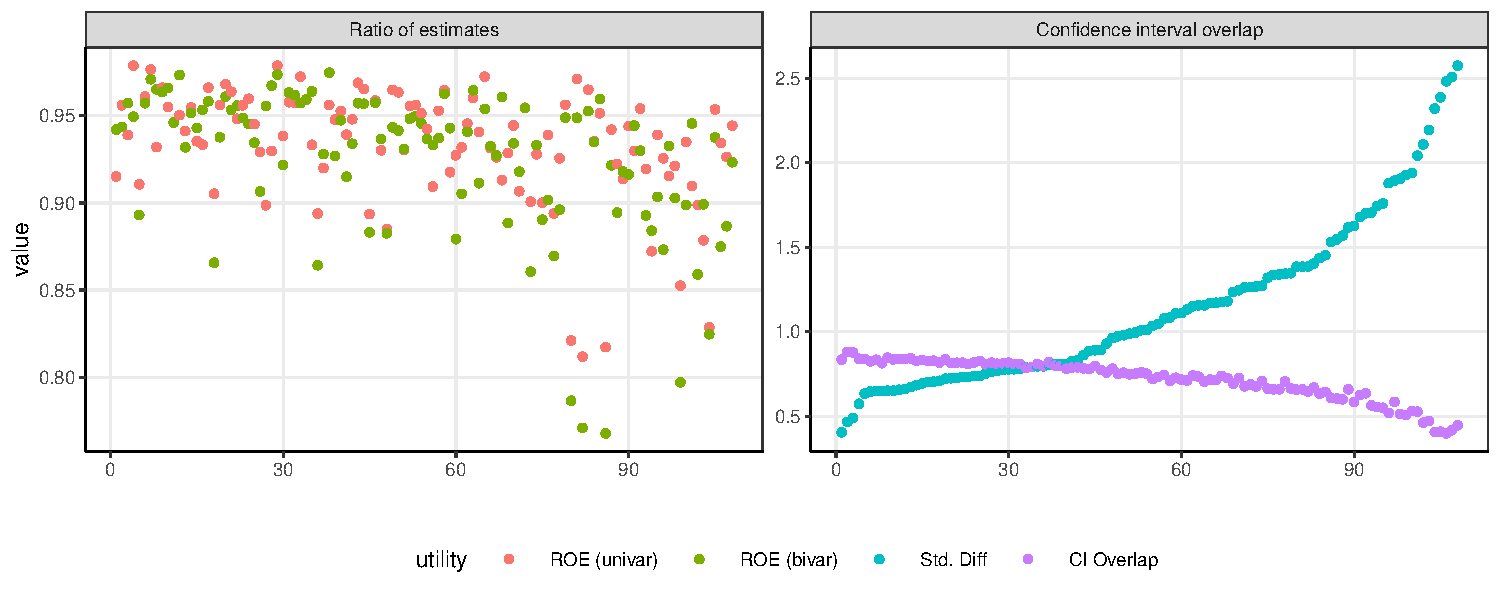
\includegraphics{../../simulation_data/categorical/graphs/ctgan/graph_compare_ctgan_utility.pdf}}
    \label{graph_compare_utility_sim_categorical_ctgan}
\end{figure}
}

\frame{\frametitle{Estimating utility in CTGAN (model \ref{model_1})}
\vspace{-5mm}
\begin{figure}
    \caption{Parametric estimates from linear model}
    \vspace{-5mm}
    \resizebox{\textwidth}{!}{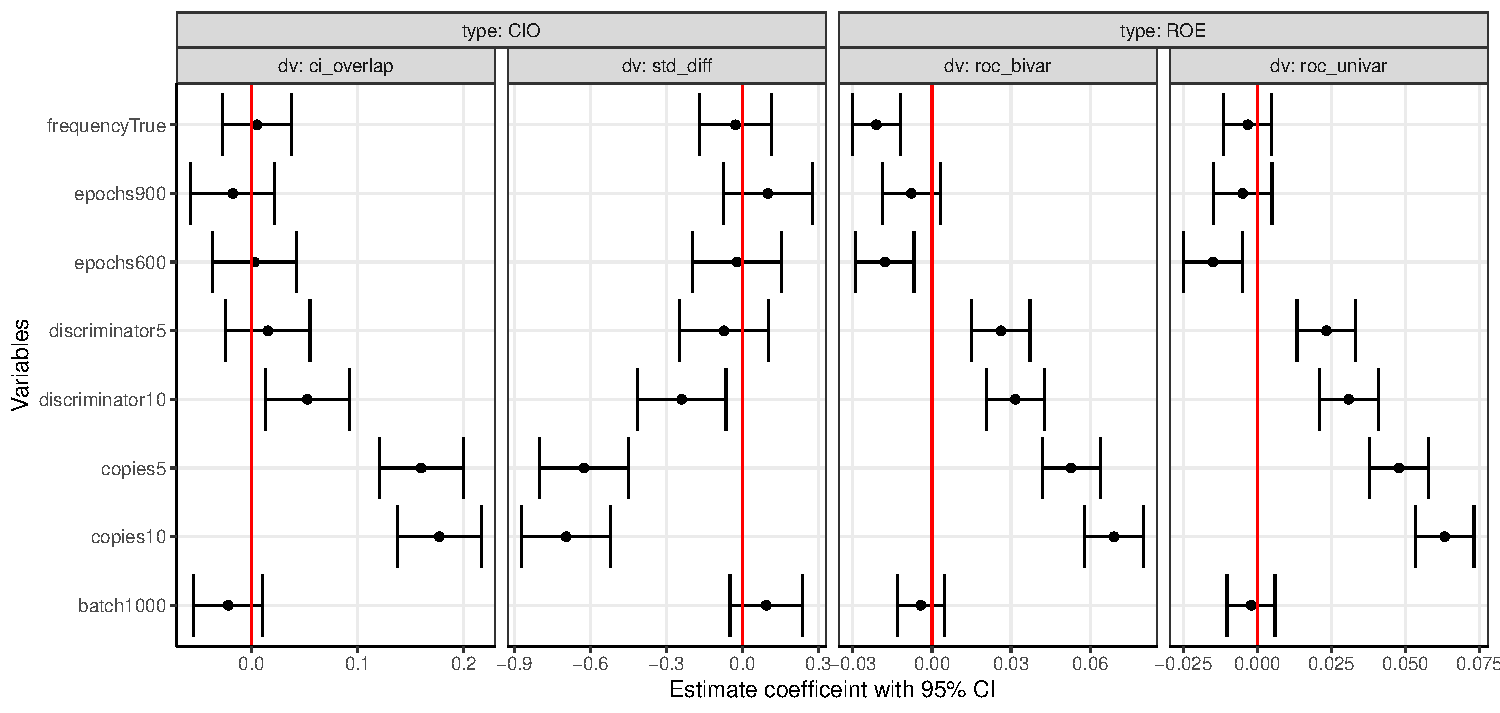
\includegraphics{../../simulation_data/categorical/graphs/ctgan/graph_ctgan_utility_compare.pdf}}
    \label{graph_ctgan_utility_compare}
\end{figure}
}

\frame{\frametitle{Estimating utility in CTGAN by copies ($m$)  (model \ref{model_2})}
\vspace{-5mm}
\begin{figure}
    \caption{Parametric estimates from linear model}
    \vspace{-5mm}
    \resizebox{\textwidth}{!}{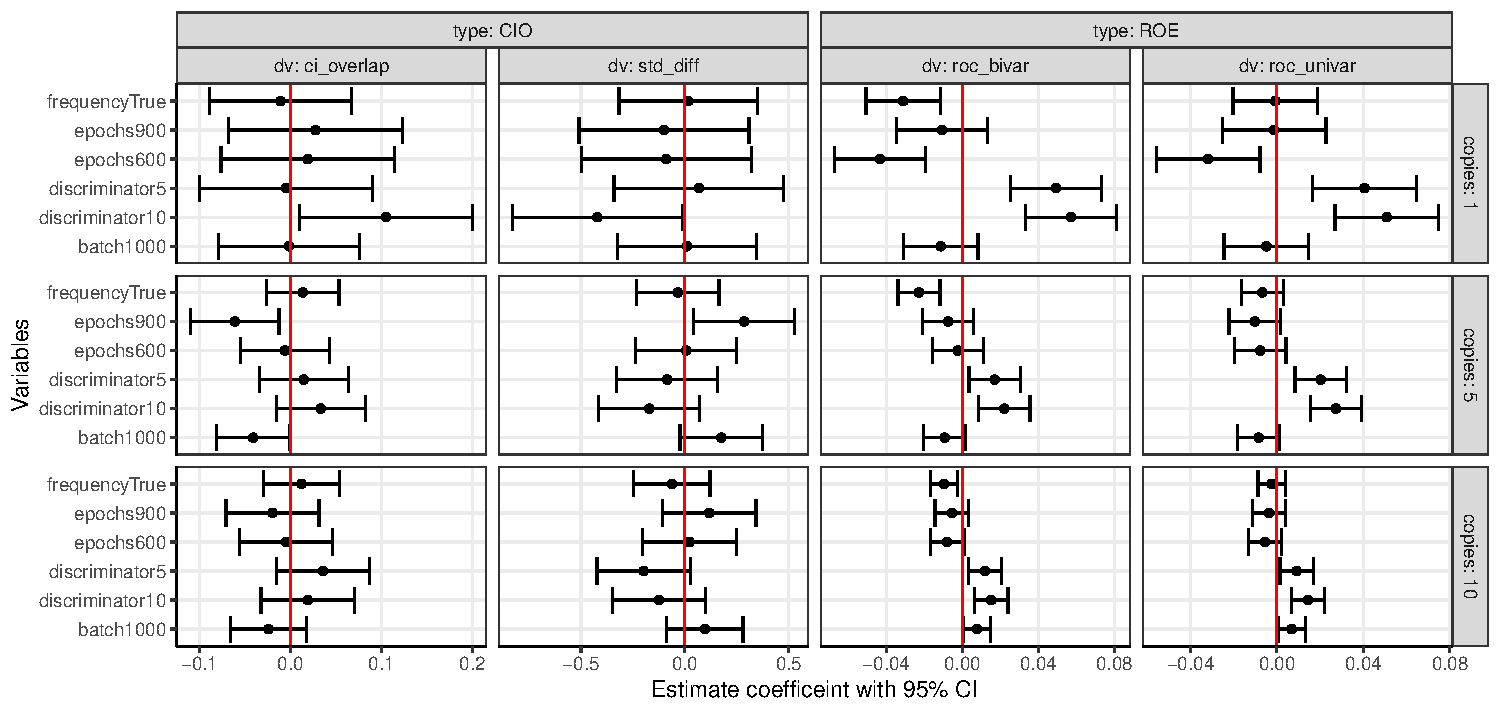
\includegraphics{../../simulation_data/categorical/graphs/ctgan/graph_ctgan_utility_compare_copies.pdf}}
    \label{graph_ctgan_utility_compare_copies}
\end{figure}
}


\frame{\frametitle{Compare frequency counts between baseline and tuned}
\vspace{-5mm}
\begin{figure}
    \caption{}
    \resizebox{\textwidth}{!}{\includegraphics{../../simulation_data/categorical/graphs/graph_compare_frequency.pdf}}
    \label{graph_compare_frequency_categorical}
\end{figure}
}

\frame{\frametitle{Compare regression output between baseline and tuned}
\vspace{-5mm}
\begin{figure}
    \caption{}
    \resizebox{\textwidth}{!}{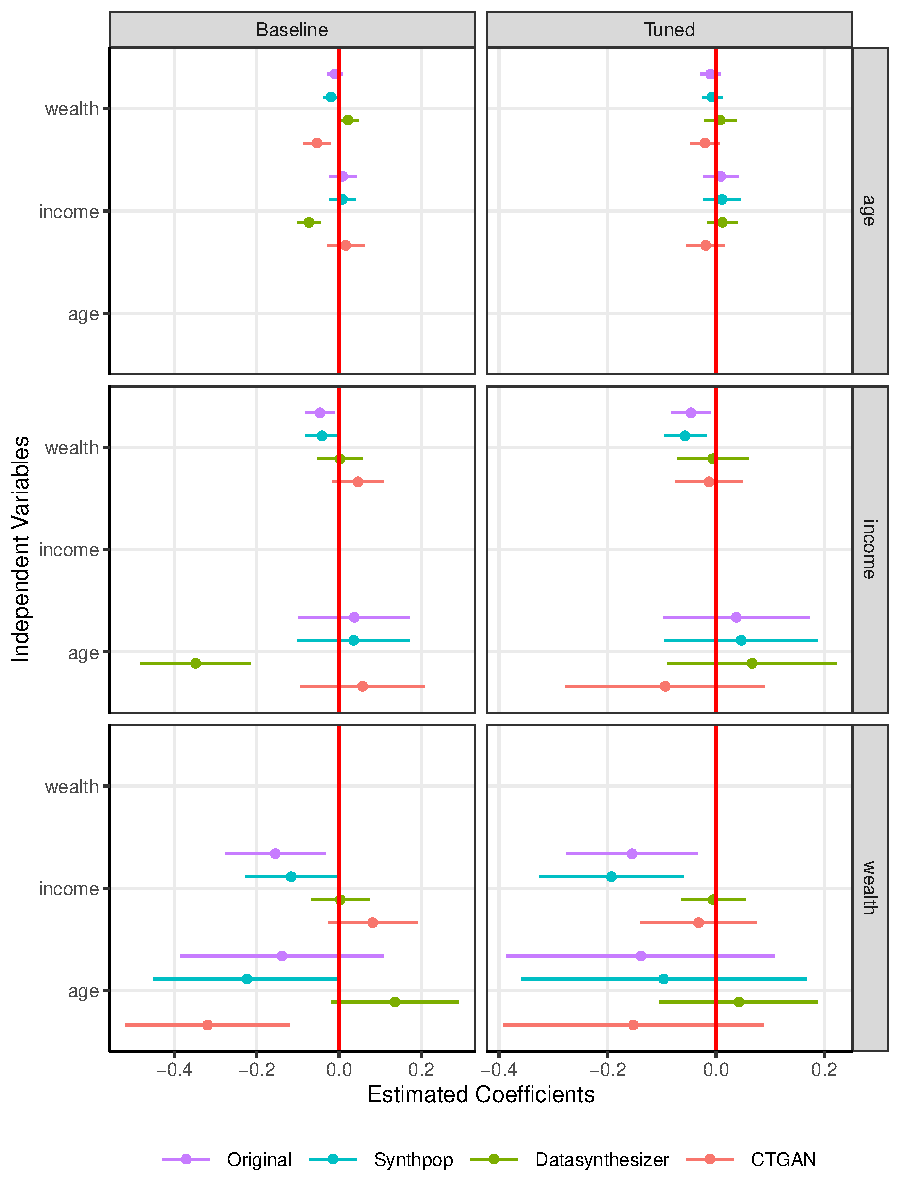
\includegraphics{../../simulation_data/categorical/graphs/graph_compare_cio_regressions.pdf}}
    \label{graph_compare_cio_regressions_categorical}
\end{figure}
}


\frame{\frametitle{Measuring utility for simulated categorical data}
\vspace{-5mm}
\begin{figure}
    \caption{}
    \resizebox{\textwidth}{!}{\includegraphics{../../simulation_data/categorical/graphs/graph_compare_utility.pdf}}
    \label{graph_compare_utility_sim_categorical}
\end{figure}
}

\frame{\frametitle{Summary: Synthpop has highest utility}
\begin{table}[h]
\caption{Comparison of Results}
\label{table_comparison}
\centering
\begin{tabular}{lrrrr}
\toprule
Data                            & ROE univar & ROE bivar & Std. Diff & CIO \\
\midrule
Simulated categorical variables & =          & =         & SP        & SP \\
\bottomrule
\end{tabular}
\end{table}
\begin{itemize}
    \item CTGAN/Datasynthesizer requires tuning (not Synthpop)
    \item Unexpectedly, CTGAN performs 2nd best for categorical data
\end{itemize}
}


\subsection{Simulated continuous data}\label{sec_results_continuous}
\frame[c]{\frametitle{}
\centering
Section \ref{sec_results}: Results \\
Section \ref{sec_results}\ref{sec_results_continuous}: Simulated continuous data
}

\frame{\frametitle{Descriptive statistics - continuous variables}
\begin{table}[!h]
    \caption{}
    \centering
    \resizebox{\textwidth}{!}{\begin{tabular}{rlrrrrr}
\toprule
number & variable & min & max & mean & std & median \\
\midrule
1 & age & 16.00 & 94.00 & 55.65 & 22.56 & 57.00 \\
2 & income & 624.00 & 349355.00 & 35721.10 & 41455.86 & 22421.50 \\
3 & wealth & -19560.00 & 89975356.00 & 659520.71 & 3165853.95 & 127616.00 \\
\bottomrule
\end{tabular}
}
    \label{table_variables_continuous}
\end{table}
}

\frame{\frametitle{Measuring utility for simulated continuous data}
\vspace{-5mm}
\begin{figure}
    \caption{}
    \resizebox{\textwidth}{!}{\includegraphics{../../simulation_data/continuous/graphs/graph_compare_utility.pdf}}
    \label{graph_compare_utility_sim_continuous}
\end{figure}
}

\frame{\frametitle{Summary: Synthpop has highest levels of utility}
\begin{table}[h]
\caption{Comparison of Results}
\label{table_comparison}
\centering
\begin{tabular}{lrrrr}
\toprule
Data                            & ROE univar & ROE bivar & Std. Diff & CIO \\
\midrule
Simulated continuous variables  & SP         & =         & SP        & SP \\
\bottomrule
\end{tabular}
\end{table}
\begin{itemize}
    \item CTGAN has similar level of CIO but higher Std. Diff
    \item Datasynthesizer performs the worst, as we would expect given dataset with only continuous variables
\end{itemize}
}


\subsection{UK 1991}\label{sec_results_UK1991}
\frame[c]{\frametitle{}
\centering
Section \ref{sec_results}: Results \\
Section \ref{sec_results}\ref{sec_results_UK1991}: Individual Sample of Anonymised Records (SAR) for the British Census, subsetted on the region of West Midlands (UK 1991)
}

\frame{\frametitle{Descriptive statistics - UK 1991}
\vspace{-5mm}
\begin{figure}
    \caption{}
    \vspace{-5mm}
    \resizebox{\textwidth}{!}{\includegraphics{../../UK1991/graphs/graph_descriptives.pdf}}
    \label{graph_descriptives}
\end{figure}
}

\frame{\frametitle{Measuring utility}
\vspace{-5mm}
\begin{figure}
    \caption{Ratio of estimates}
    \resizebox{\textwidth}{!}{\includegraphics{../../UK1991/graphs/graph_compare_utility_roe.pdf}}
    \label{graph_compare_utility_roe}
\end{figure}
}

\frame{\frametitle{Measuring utility}
\vspace{-5mm}
\begin{figure}
    \caption{Confidence interval overlap}
\vspace{-5mm}
    \resizebox{\textwidth}{!}{\includegraphics{../../UK1991/graphs/graph_compare_utility_cio.pdf}}
    \label{graph_compare_utility_cio}
\end{figure}
}

% \frame{\frametitle{Frequency statistics}
% \vspace{-5mm}
% \begin{figure}
%     \caption{}
%     \vspace{-5mm}
%     \resizebox{\textwidth}{!}{\includegraphics{../../UK1991/graphs/graph_compare_frequency.pdf}}
%     \label{graph_compare_frequency}
% \end{figure}
% }

% \frame{\frametitle{Regression (DV: MSTATUS - married vs. single)}
% \vspace{-5mm}
% \begin{figure}
%     \caption{CTGAN is closest to original}
%     \vspace{-5mm}
%     \resizebox{\textwidth}{!}{\includegraphics{../../UK1991/graphs/graph_compare_cio_mstatus.pdf}}
%     \label{graph_compare_cio_mstatus}
% \end{figure}
% }

% \frame{\frametitle{Regression (DV: TENURE - own vs. rent)}
% \vspace{-5mm}
% \begin{figure}
%     \caption{Synthpop is closest to original}
%     \vspace{-5mm}
%     \resizebox{\textwidth}{!}{\includegraphics{../../UK1991/graphs/graph_compare_cio_tenure.pdf}}
%     \label{graph_compare_cio_tenure}
% \end{figure}
% }

\frame{\frametitle{Comparing duration to create 1 synthetic data set ($\times5$)}
\begin{table}[!h]
    \caption{UK 1991 data, 12 variables (1 continuous), and  $\approx$ 20.000 observations}
    \centering
    \input{../../UK1991/tables/duration/table_duration.tex}
    % \resizebox{\textwidth}{!}{\input{../../UK1991/tables/duration/table_duration.tex}}
    \label{table_dution_UK1991}
\end{table}
}

\frame{\frametitle{Summary: things become more complicated in `real' data}
\begin{table}[h]
\caption{Comparison of Results}
\label{table_comparison}
\centering
\begin{tabular}{lrrrr}
\toprule
Data                            & ROE univar & ROE bivar & Std. Diff & CIO \\
\midrule
UK1991                          & (1) DS/ (2) CTGAN   & (1) DS/ (2) SP     &           & \\
\hskip 5mm DV: MSTATUS          &            &           & CTGAN     & CTGAN \\
\hskip 5mm DV: TENURE           &            &           & SP        & SP \\
\bottomrule
\end{tabular}
\end{table}

}

\subsection{SD 2011}\label{sec_results_SD2011}
\frame[c]{\frametitle{}
\centering
Section \ref{sec_results}: Results \\
Section \ref{sec_results}\ref{sec_results_SD2011}: Social Diagnosis 2011 (SD2011)
}

\frame{\frametitle{Descriptive statistics - SD2011}
\vspace{-5mm}
\begin{figure}
    \caption{}
    \resizebox{\textwidth}{!}{\includegraphics{../../SD2011/graphs/graph_descriptives.pdf}}
    \label{graph_descriptives}
\end{figure}
}

\frame{\frametitle{Measuring utility}
\vspace{-5mm}
\begin{figure}
    \caption{}
    \resizebox{\textwidth}{!}{\includegraphics{../../SD2011/graphs/graph_compare_utility.pdf}}
    \label{graph_compare_utility}
\end{figure}
}

% \frame{\frametitle{Frequency statistics}
% \vspace{-5mm}
% \begin{figure}
%     \caption{}
%     \vspace{-5mm}
%     \resizebox{\textwidth}{!}{\includegraphics{../../SD2011/graphs/graph_compare_frequency.pdf}}
%     \label{graph_compare_frequency}
% \end{figure}
% }

% \frame{\frametitle{Confidence interval overlap (DV: LN Income)}
% \vspace{-5mm}
% \begin{figure}
%     \caption{}
%     \resizebox{\textwidth}{!}{\includegraphics{../../SD2011/graphs/graph_compare_cio.pdf}}
%     \label{graph_compare_cio}
% \end{figure}
% }

\frame{\frametitle{Comparing duration to create 1 synthetic data set ($\times5$)}
\begin{table}[!h]
    \caption{SD 2011, 4 variables (2 continuous), and $\approx$ 5.000 observations}
    \centering
    \input{../../SD2011/tables/duration/table_duration.tex}
    % \resizebox{\textwidth}{!}{\input{../../UK1991/tables/duration/table_duration.tex}}
    \label{table_dution_SD2011}
\end{table}

$^*$ Synthpop $<$ 1 second
}


\frame{\frametitle{Summary}
\begin{itemize}
        \item Synthpop is the best (ROE/CIO)
    \item CTGAN is slowest 
\end{itemize}
}

\section{Conclusion}\label{sec_conclusion}
\frame[c]{\frametitle{}
\centering
Section \ref{sec_conclusion}: Conclusion
}

\frame{\frametitle{Summary}
\begin{table}[h]
\caption{Comparison of Results}
\label{table_comparison}
\centering
\begin{tabular}{lrrrr}
\toprule
Data                            & ROE univar & ROE bivar & Std. Diff & CIO \\
\midrule
Simulated categorical variables & =          & =         & SP        & SP \\
Simulated continuous variables  & SP         & =         & SP        & SP \\
UK1991                          & DS/CTGAN   & DS/SP     &           & \\
\hskip 5mm DV: MSTATUS          &            &           & CTGAN     & CTGAN \\
\hskip 5mm DV: TENURE           &            &           & SP        & SP \\
SD2011                          & =          & =         & SP        & SP \\
\bottomrule
\end{tabular}
\end{table}
}



\frame{\frametitle{Results}
\begin{itemize}
        \item Main message: Synthpop is the `winner'
    \begin{itemize}
                \item However, it is not always the `best'
        \item Easy - little tuning required 
        \item Fastest
    \end{itemize}
    \item Datasynthesizer
    \begin{itemize}
                \item Requires tuning
        \item Struggles with continuous variables
    \end{itemize}
    \item CTGAN
    \begin{itemize}
                \item Requires tuning
        \item Struggles with categorical variables
        \item Slowest
    \end{itemize}
\end{itemize}
}

\frame{\frametitle{Next steps}
\begin{itemize}
        \item What determines which package is better?
    \item Simulation data
    \begin{itemize}
                \item Mixed data (categorical and continuous)
        \item Correlated variables
        \item Missing values 
    \end{itemize}
    \item Real data
    \begin{itemize}
                \item Dimensions (number, type of variables) 
    \end{itemize}
    \item Different measures of utility
    \item Different packages for creating synthetic data
    \item Privacy
\end{itemize}
}


\frame[c]{\frametitle{}
\centering
Thank you
}


\end{spacing}

\end{document}

